\documentclass[tikz,border=10pt]{standalone}
\usepackage{tikz}
\usepackage{amsmath,amssymb}
\usetikzlibrary{shapes,arrows.meta,positioning,calc,fit,backgrounds,decorations.pathreplacing}

\begin{document}
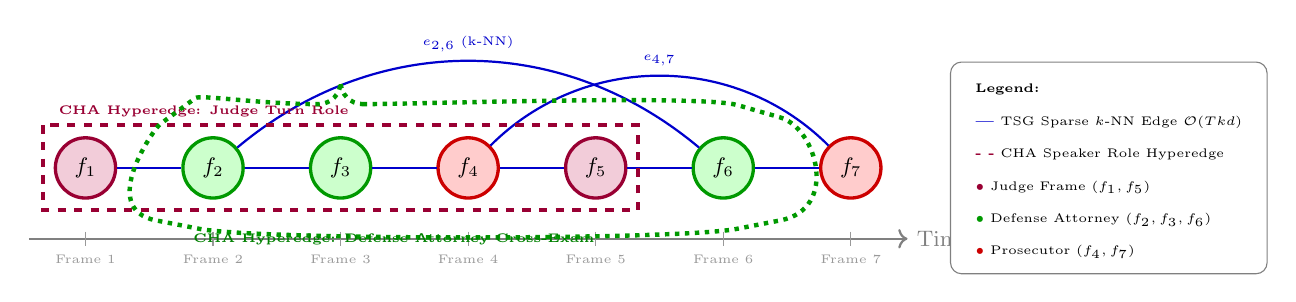
\begin{tikzpicture}[
    scale=0.9,
    every node/.style={transform shape},
    frame/.style={draw=black!80, circle, fill=blue!15, line width=1.0pt, minimum size=0.8cm, font=\small\bfseries},
    spk_judge/.style={draw=purple!80!black, circle, fill=purple!20, line width=1.2pt, minimum size=0.85cm, font=\small\bfseries},
    spk_def/.style={draw=green!60!black, circle, fill=green!20, line width=1.2pt, minimum size=0.85cm, font=\small\bfseries},
    spk_pros/.style={draw=red!80!black, circle, fill=red!20, line width=1.2pt, minimum size=0.85cm, font=\small\bfseries}
]

    % Frame nodes across time axis
    \node[spk_judge] (f1) at (0, 0) {$f_1$};
    \node[spk_def] (f2) at (1.8, 0) {$f_2$};
    \node[spk_def] (f3) at (3.6, 0) {$f_3$};
    \node[spk_pros] (f4) at (5.4, 0) {$f_4$};
    \node[spk_judge] (f5) at (7.2, 0) {$f_5$};
    \node[spk_def] (f6) at (9.0, 0) {$f_6$};
    \node[spk_pros] (f7) at (10.8, 0) {$f_7$};

    % Time axis line below
    \draw[thick,->, black!50] (-0.8, -1.0) -- (11.6, -1.0) node[right, font=\small] {Timeline $t$};
    
    \foreach \x/\lbl in {0/1, 1.8/2, 3.6/3, 5.4/4, 7.2/5, 9.0/6, 10.8/7} {
        \draw[black!40] (\x, -0.9) -- (\x, -1.1) node[below, font=\tiny] {Frame \lbl};
    }

    % TSG 1D Local & Sparse k-NN Edges (Blue Solid Lines)
    \draw[thick, blue!80!black] (f1) -- (f2);
    \draw[thick, blue!80!black] (f2) -- (f3);
    \draw[thick, blue!80!black] (f3) -- (f4);
    \draw[thick, blue!80!black] (f4) -- (f5);
    \draw[thick, blue!80!black] (f5) -- (f6);
    \draw[thick, blue!80!black] (f6) -- (f7);

    % TSG k-NN Long-Range Similarity Edges
    \draw[thick, blue!80!black, bend left=40] (f2) to node[above, font=\tiny, blue!80!black] {$e_{2,6}$ (k-NN)} (f6);
    \draw[thick, blue!80!black, bend left=45] (f4) to node[above, font=\tiny, blue!80!black] {$e_{4,7}$} (f7);

    % CHA Hyperedges (Dashed Speaker Role Enclosures)
    % Judge Hyperedge (f1, f5)
    \draw[dashed, line width=1.4pt, purple!80!black] 
        ($(f1.center)+(-0.6,0.6)$) rectangle ($(f5.center)+(0.6,-0.6)$);
    \node[purple!80!black, font=\tiny\bfseries, anchor=south west] at ($(f1.center)+(-0.5,0.6)$) {CHA Hyperedge: Judge Turn Role};

    % Defense Attorney Hyperedge (f2, f3, f6)
    \draw[dotted, line width=1.6pt, green!60!black] 
         plot [smooth cycle, rounded corners=8pt] coordinates {
            ($(f2.center)+(-0.5, 0.8)$) 
            ($(f3.center)+(0.0, 0.9)$) 
            ($(f6.center)+(0.5, 0.8)$) 
            ($(f6.center)+(0.5, -0.8)$) 
            ($(f2.center)+(-0.5, -0.8)$)
         };
    \node[green!50!black, font=\tiny\bfseries, anchor=north west] at ($(f2.center)+(-0.4,-0.8)$) {CHA Hyperedge: Defense Attorney Cross-Exam};

    % Legend Box
    \node[draw=black!50, fill=white, rounded corners=4pt, anchor=west, inner sep=4pt] at (12.2, 0) {
        \begin{tabular}{l}
            \tiny\textbf{Legend:}\\[1pt]
            \tiny \textcolor{blue!80!black}{\textbf{---}} TSG Sparse $k$-NN Edge $\mathcal{O}(Tkd)$\\[1pt]
            \tiny \textcolor{purple!80!black}{\textbf{- -}} CHA Speaker Role Hyperedge\\[1pt]
            \tiny \textcolor{purple!80!black}{$\bullet$} Judge Frame ($f_1, f_5$)\\[1pt]
            \tiny \textcolor{green!60!black}{$\bullet$} Defense Attorney ($f_2, f_3, f_6$)\\[1pt]
            \tiny \textcolor{red!80!black}{$\bullet$} Prosecutor ($f_4, f_7$)
        \end{tabular}
    };

\end{tikzpicture}
\end{document}
